% flashcards-title: Three rising trend lines on separate axes
% flashcards-desc: Three small graphs labeled A, B, and C, each with a horizontal and a vertical axis meeting at a corner marked zero. In A a straight line rises from the corner itself. In B a straight line rises but begins partway up the vertical axis, above the corner. In C a line leaves the corner and curves upward ever more steeply.
\documentclass[dvisvgm,tikz,border=8pt]{standalone}
\usepackage{tikz}
\usetikzlibrary{arrows.meta,calc,positioning}
\definecolor{DeckInk}{HTML}{172A3A}
\definecolor{DeckAccent}{HTML}{176B87}
\definecolor{DeckWarm}{HTML}{D97706}
\definecolor{DeckMuted}{HTML}{667784}
\definecolor{DeckPaper}{HTML}{F7FAFC}
\tikzset{
  every node/.style={font=\sffamily, text=DeckInk},
  object/.style={draw=DeckInk, line width=1.1pt, fill=DeckPaper},
  primary/.style={draw=DeckAccent, line width=1.5pt},
  boundary/.style={draw=DeckAccent, line width=1.5pt, dashed, rounded corners=6pt},
  guide/.style={draw=DeckMuted, line width=0.9pt, dashed},
  dimension/.style={{Stealth[length=3.2mm,width=2.2mm]}-{Stealth[length=3.2mm,width=2.2mm]}, draw=DeckWarm, line width=1.2pt},
  motion/.style={-{Stealth[length=3.5mm,width=2.5mm]}, draw=DeckAccent, line width=1.5pt, dashed},
}

\begin{document}
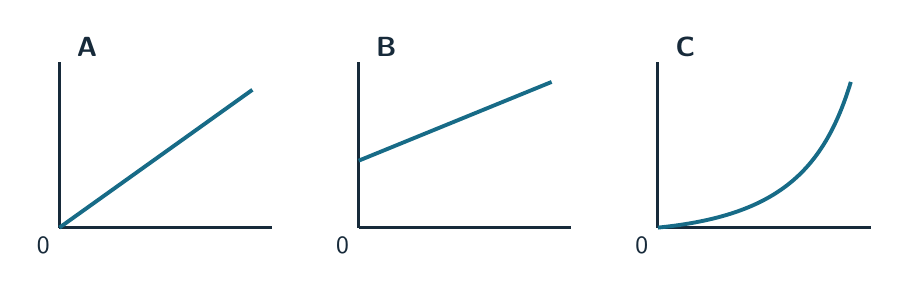
\begin{tikzpicture}[x=1cm,y=1cm]
  % Panel A: straight through the origin
  \draw[DeckInk, line width=1.1pt] (0,0) -- (2.7,0);
  \draw[DeckInk, line width=1.1pt] (0,0) -- (0,2.1);
  \node[font=\sffamily\small, below left=0pt and 0pt of {(0,0)}] {0};
  \node[font=\sffamily\bfseries] at (0.35,2.3) {A};
  \draw[DeckAccent, line width=1.4pt] (0,0) -- (2.45,1.75);
  % Panel B: straight, nonzero start
  \begin{scope}[xshift=3.8cm]
    \draw[DeckInk, line width=1.1pt] (0,0) -- (2.7,0);
    \draw[DeckInk, line width=1.1pt] (0,0) -- (0,2.1);
    \node[font=\sffamily\small, below left=0pt and 0pt of {(0,0)}] {0};
    \node[font=\sffamily\bfseries] at (0.35,2.3) {B};
    \draw[DeckAccent, line width=1.4pt] (0,0.85) -- (2.45,1.85);
  \end{scope}
  % Panel C: through the origin but curving upward
  \begin{scope}[xshift=7.6cm]
    \draw[DeckInk, line width=1.1pt] (0,0) -- (2.7,0);
    \draw[DeckInk, line width=1.1pt] (0,0) -- (0,2.1);
    \node[font=\sffamily\small, below left=0pt and 0pt of {(0,0)}] {0};
    \node[font=\sffamily\bfseries] at (0.35,2.3) {C};
    \draw[DeckAccent, line width=1.4pt]
      (0,0) .. controls (1.5,0.15) and (2.1,0.7) .. (2.45,1.85);
  \end{scope}
\end{tikzpicture}
\end{document}
